\section{GoF Patterns}

\subsection{Factory Method (Creational)}

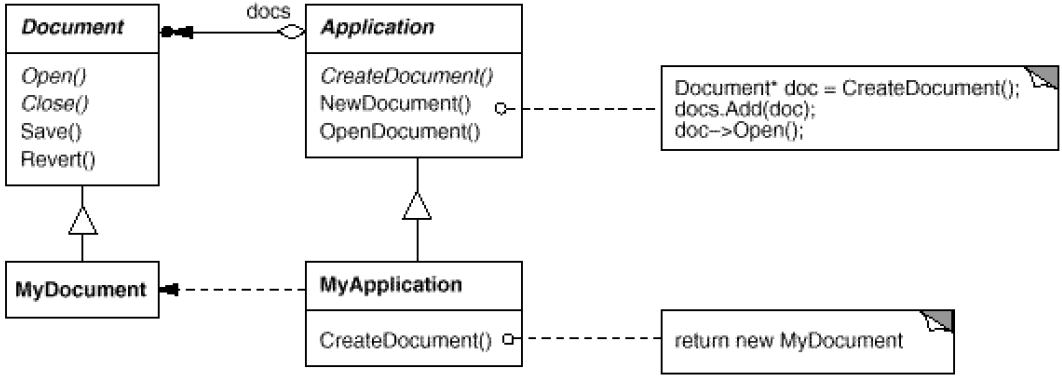
\includegraphics[width=\linewidth]{factory_method.png}

Bietet eine Schnittstelle um in der Super-Klasse neue Objekte erstellen zu können, aber erlaubt den Sub-Klassen den Typ zu verändern der erstellt werden soll

\subsubsection{Consequences}

\textbf{Benefits}
\begin{itemize}
    \item Verhindert enge Kopplung zwischen dem Creator und dem konkreten Produkt
    \item \textcolor{blue}{Single Responsibility Principle} Der Product Creation Code kann einfach herumgeschoben werden $\rightarrow$ Macht den Support einfacher
    \item \textcolor{blue}{Open / Closed Principle} Es können neue Produkt-Typen hinzugefügt werden, ohne den Client Code zu zerstören
\end{itemize}
\vspace{10pt}
\textbf{Liabilities}
\begin{itemize}
    \item Code kann komplizierter werden, weil viele Sub-Klassen erstellt werden müssen
\end{itemize}

\subsection{Abstract Factory (Creational)}

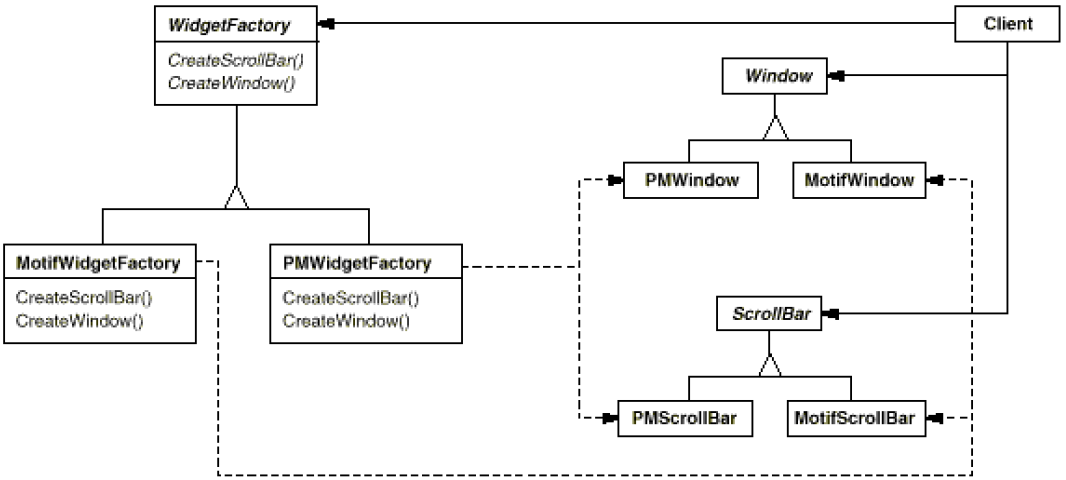
\includegraphics[width=\linewidth]{abstract_factory.png}

Erlaubt das Erstellen von Familien verwandter Objekte, ohne dessen konkrete Klasse zu spezifizieren

\subsubsection{Consequences}

\textbf{Benefits}
\begin{itemize}
    \item Man kann sicher sein, dass die Produkte einer Factory miteinander kompatible sind
    \item Vermeidet enge Kopplung zwischen konkreten Produkten und Client Code
    \item \textcolor{blue}{Single Responsibility Principle} Der Product Creation Code kann einfach herumgeschoben werden $\rightarrow$ Macht den Support einfacher
    \item \textcolor{blue}{Open / Closed Principle} Es können neue Varianten hinzugefügt werden ohne existierenden Code
    zu zerstören
\end{itemize}
\vspace{10pt}
\textbf{Liabilities}

\begin{itemize}
    \item Der Code kann komplizierter werden, als er sein sollte, weil viele neue Interfaces und Klassen erstellt werden mit dem Pattern
\end{itemize}

\subsection{Prototype (Creational)}

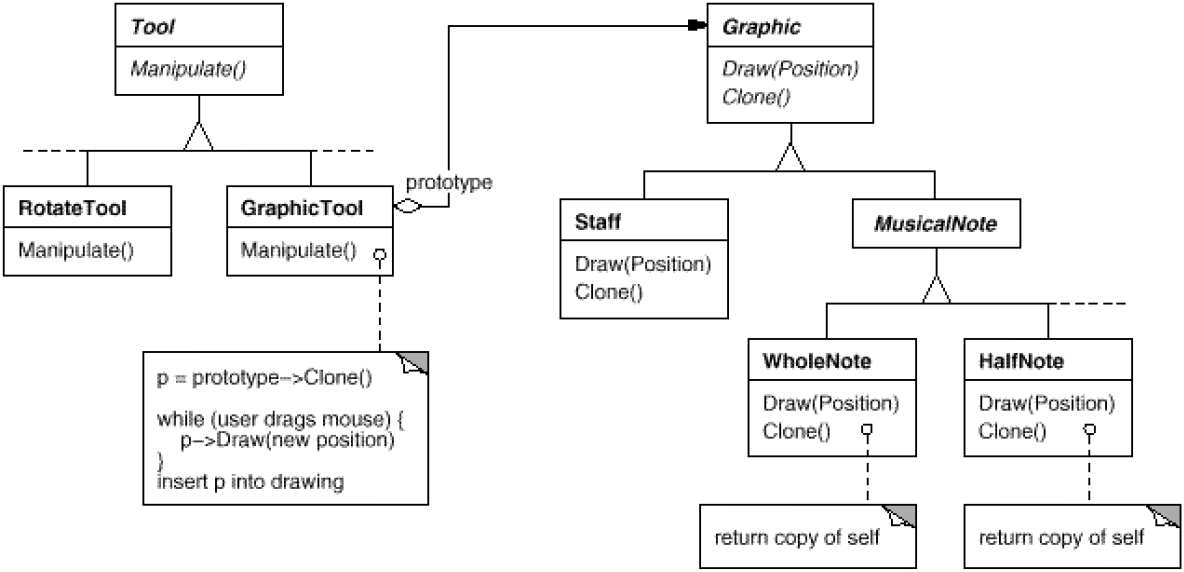
\includegraphics[width=\linewidth]{prototype.png}

Erlaubt das Kopieren existierender Objekte ohne dass der Code abhängig der Klasse wird

\subsubsection{Consequences}

\textbf{Benefits}
\begin{itemize}
    \item Objekte können geklont werden, ohne Kopplung zu dessen konkreter Klasse
    \item Wiederholte Initialisierung kann durch das Klonen vermieden werden
    \item Komplexe Objekte können bequemer erstellt werden
    \item Alternative von Vererbung beim Umgang mit Voreinstellungen für komplexe Objekte
\end{itemize}
\vspace{10pt}
\textbf{Liabilities}

\begin{itemize}
    \item Sehr tricky Objekte mit zirkularen Referenzen zu klonen
\end{itemize}

\subsection{Composite (Structural)}

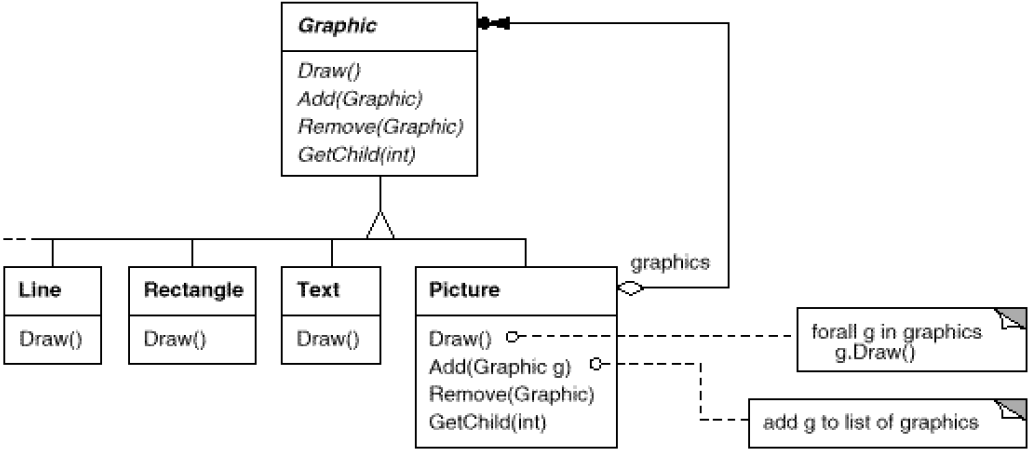
\includegraphics[width=\linewidth]{composite.png}
\textit{* Schwarzer Pfeil sollte Stern sein} \\

Stelle \textcolor{blue}{Objekte in einer Baumstruktur} zusammen um Hierarchien darzustellen. Lässt einzelne Objekte und Zusammenstellung von mehreren Objekten einheitlich behandeln

\subsubsection{Consequences}

\textbf{Benefits}
\begin{itemize}
    \item Bequemer um mit komplexen Baumstrukturen zu arbeiten. Verwende Polymorphismus und Rekursion zum Vorteil
    \item \textcolor{blue}{Open / Closed Principle} Es können neue Element-Typen hinzugefügt werden, ohne den existierenden Code zu zerstören
\end{itemize}
\vspace{10pt}
\textbf{Liabilities}

\begin{itemize}
    \item Es kann schwierig sein, eine gemeinsame Schnittstelle anzubieten
\end{itemize}

\subsection{Decorator (Wrapper) (Structural)}

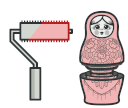
\includegraphics[width=0.25\linewidth]{decorator-icon.png}

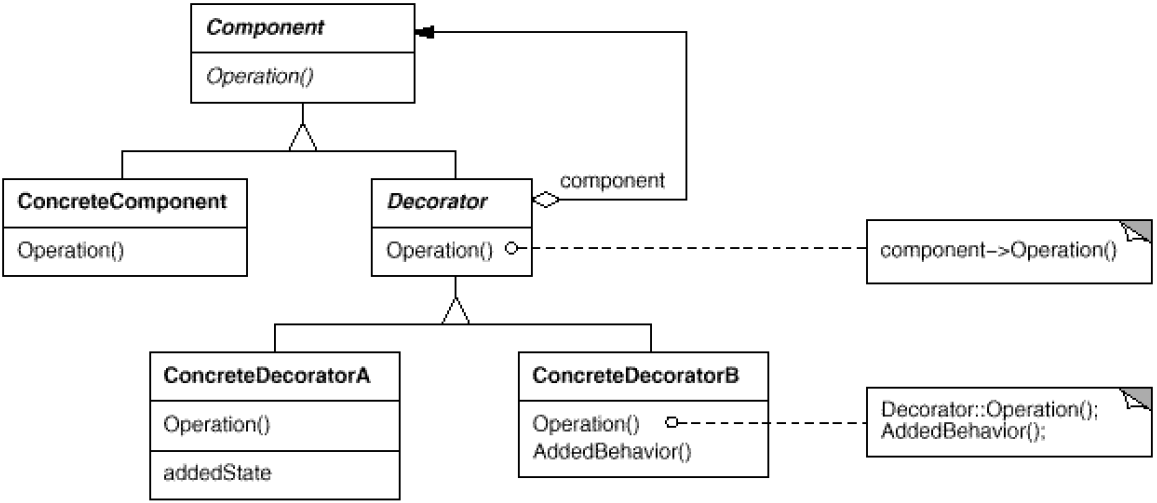
\includegraphics[width=\linewidth]{decorator.png}

Erlaubt dynamisch einem Objekt zusätzliches Verhalten hinzuzufügen, indem diese in ein Wrapper gesetzt
werden

\subsubsection{Consequences}

\textbf{Benefits}
\begin{itemize}
    \item Das Verhalten eines Objekts kann erweitert werden, ohne Sub-Klassen zu erstellen
    \item Verantwortungen können zur Laufzeit einem Objekt hinzugefügt und entfernt werden
    \item Mehrere Verhalten können kombiniert werden, indem ein Objekt in mehrere Decorator gewrappt wird
    \item \textcolor{blue}{Single Responsibility Principle} Ein Monolith kann in mehrere kleine Klassen unterteilt werden
\end{itemize}
\vspace{10pt}
\textbf{Liabilities}

\begin{itemize}
    \item Es ist schwer ein Wrapper vom Wrapper-Stack zu entfernen
    \item Es ist schwer ein Decorator so zu implementieren, dass die Reihenfolge keine Rolle spielt
    \item Der initiale Configurations Code von Layers kann hässlich aussehen
\end{itemize}

\subsection{Adapter (Structural)}

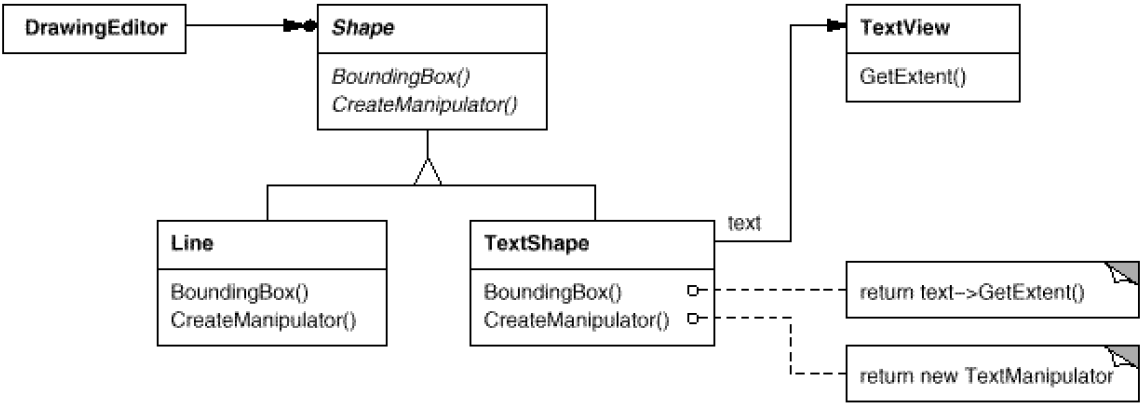
\includegraphics[width=\linewidth]{adapter.png}

Erlaubt Objekten mit inkompatiblen Schnittstellen zusammenzuarbeiten

\subsubsection{Consequences}

\textbf{Benefits}
\begin{itemize}
    \item \textcolor{blue}{Single Responsibility Principle} Das Interface oder Data Conversion Code kann von der Business Logik separiert werden
    \item \textcolor{blue}{Open / Closed Principle} Es können neue Adapters hinzugefügt werden, ohne den Client Code zu zerstören
\end{itemize}
\vspace{10pt}
\textbf{Liabilities}

\begin{itemize}
    \item Die Gesamt-Komplexität des Codes steigt, weil neue Interfaces und Klassen erstellt werden müssen
\end{itemize}

\subsection{Proxy}

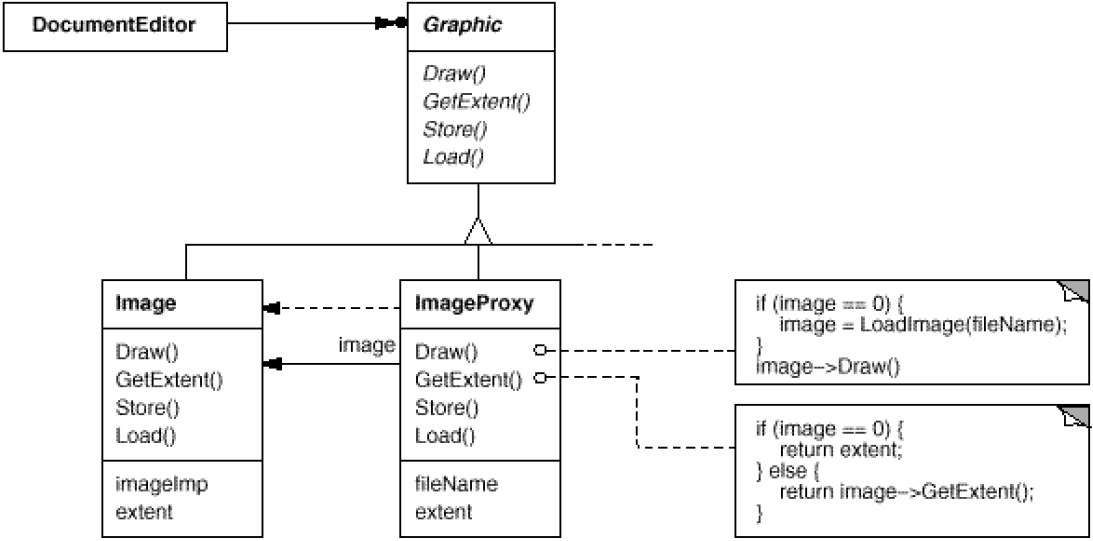
\includegraphics[width=\linewidth]{proxy.png}

Bietet einen Stellvertreter oder Platzhalter für ein anderes Objekt. Ein Proxy kontrolliert den Zugriff auf das originial Objekt, was erlaubt vor oder nach dem eigentlichen Request, Code auszuführen.

\subsubsection{Consequences}

\textbf{Benefits}
\begin{itemize}
    \item Das Service Objekt kann kontrolliert werden, ohne das der Client etwas davon weiss
    \item Ermöglicht das managen des Life-Cycles des Services wenn sich Clients nicht darum kümmern
    \item Proxy funktioniert auch, wenn der Service nicht ready oder nicht verfügbar ist
    \item \textcolor{blue}{Open / Closed Principle} Neue Proxies können erstellt werden ohne den Service oder Client zu verändern
\end{itemize}
\vspace{10pt}
\textbf{Liabilities}

\begin{itemize}
    \item Code kann komplizierter werden, da neue Klassen erstellt werden müssen
    \item Antwort des Services kann verzögert werden
\end{itemize}

\subsection{Facade}

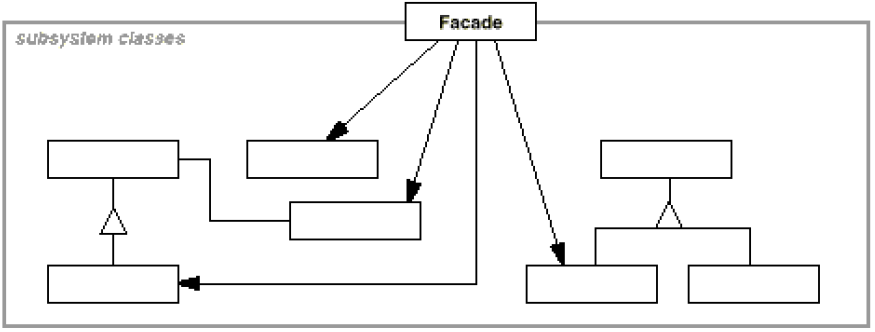
\includegraphics[width=\linewidth]{facade.png}

Stellt eine einheitliche Interface für eine Reihe von Interfaces eines Subsystems bereit. Subsysteme können Libraries, Frameworks oder ein komplexes Set von Klassen sein.

\subsubsection{Consequences}

\textbf{Benefits}
\begin{itemize}
    \item Der Code kann von der Komplexität des Subsystems isoliert werden
\end{itemize}
\vspace{10pt}
\textbf{Liabilities}

\begin{itemize}
    \item Facade kann ein God-Objekt, welches an alle Klassen einer App gekoppelt ist, werden
\end{itemize}

\subsection{Observer (Behavioral)}

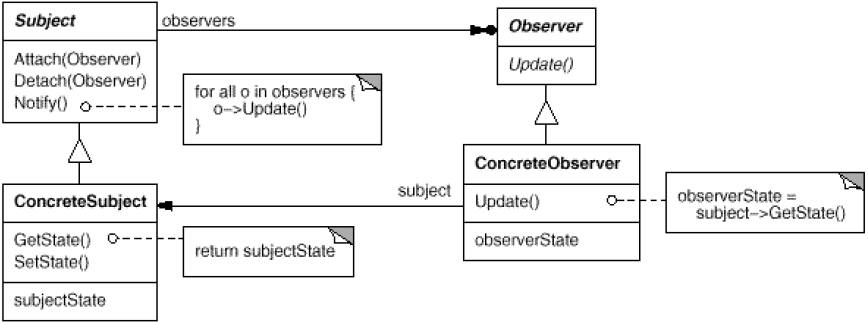
\includegraphics[width=\linewidth]{observer.png}

\subsubsection{Problem}

Anstelle, dass \textcolor{blue}{Objekt A} beim \textcolor{blue}{Objekt B} immer nachfragt, ob es sich geändert hat, benachrichtigt \textcolor{blue}{B} \textcolor{blue}{A}, dass es sich geändert hat.

\subsubsection{Solution}

Lässt einen Abonnement-Mechanismus definieren, um mehrere Objekte über alle Ereignisse zu benachrichtigen, die mit dem Objekt passieren, das sie beobachten

\subsubsection{Consequences}

\textbf{Benefits}
\begin{itemize}
    \item \textcolor{blue}{Open / Closed Principle} Es können neue Subscriber Klassen erstellt werden, ohne den Publisher
    ändern zu müssen
    \item Es können zur Laufzeit Beziehungen zwischen Objekten erstellt werden
\end{itemize}
\vspace{10pt}
\textbf{Liabilities}

\begin{itemize}
    \item Subscribers werden in zufälliger Reihenfolge benachrichtigt
\end{itemize}

\subsection{Strategy (Behavioral)}

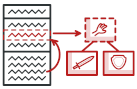
\includegraphics[width=0.25\linewidth]{strategy-icon.png}

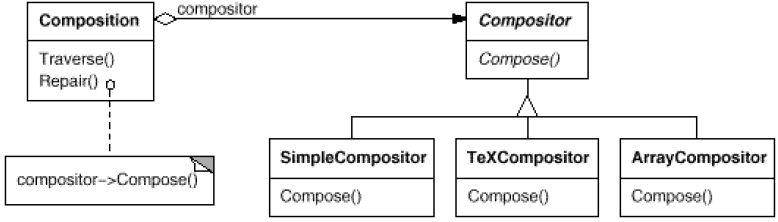
\includegraphics[width=\linewidth]{strategy.png}

\subsubsection{Problem}

Zum Beispiel unterschiedliche Algorithmen für einen Routen Planer

\subsubsection{Solution}

Lässt eine Familie von Algorithmen (für jeden Algorithmus eine eigene Klasse = Strategy) definieren und macht diese Objekte austauschbar. Strategy lässt den Algorithmus unabhängig vom Client variieren.

\subsubsection{Consequences}

\textbf{Benefits}
\begin{itemize}
    \item Algorithmen können zur Laufzeit ausgetauscht werden
    \item Isolation der Implementation Details der Algorithmen gegenüber zum Code, welcher die Algorithmen verwendet
    \item Vererbung kann mit Composition ausgetauscht werden
    \item \textcolor{blue}{Open / Closed Principle} Es können neue Strategien hinzugefügt werden, ohne den Kontext zu
    ändern
\end{itemize}
\vspace{10pt}
\textbf{Liabilities}

\begin{itemize}
    \item Überkompliziert, wenn nur wenige Algorithmen existieren und diese selten ausgetauscht werden
    \item Clients müssen die Unterschiede der Algorithmen kennen, damit der richtige ausgewählt werden
    kann
\end{itemize}

\subsection{Template Method (Behavioral)}

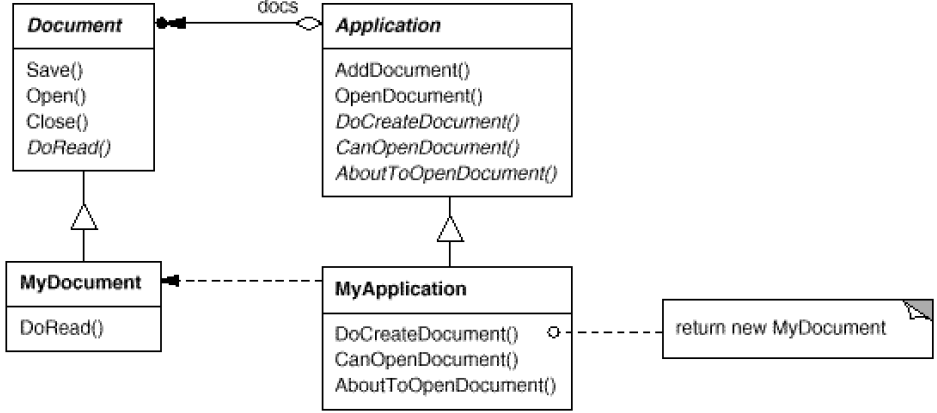
\includegraphics[width=\linewidth]{template_method.png}

\subsubsection{Problem}

Austauschen einzelner Schritte eines Workflows.

\subsubsection{Solution}

Lässt in der Super-Klasse ein Gerüst für den Algorithmus definieren, wobei Sub-Klassen gewisse Schritte des Algorithmus überschreiben können, ohne die Struktur des Algorithmus zu ändern

\subsubsection{Consequences}

\textbf{Benefits}
\begin{itemize}
    \item Clients können kleine Teile eines grossen Algorithmus austauschen
    \item Duplizierter Code kann in die Super-Klasse verschoben werden
\end{itemize}
\vspace{10pt}
\textbf{Liabilities}

\begin{itemize}
    \item Klassen können durch das bereitgestellte Gerüst limitiert werden
    \item Das \textcolor{blue}{Liskov Substitution Principle} kann verletzt werden, indem keine Default-Implementierung möglich ist
    \item Template-Methoden werden schwerer zu unterhalten, je mehr Schritte existieren
\end{itemize}

\subsection{Mediator (Vermittler) (Behavioral)}

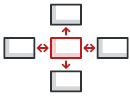
\includegraphics[width=0.2\linewidth]{mediator-icon.png}

\textbf{Static Structure}

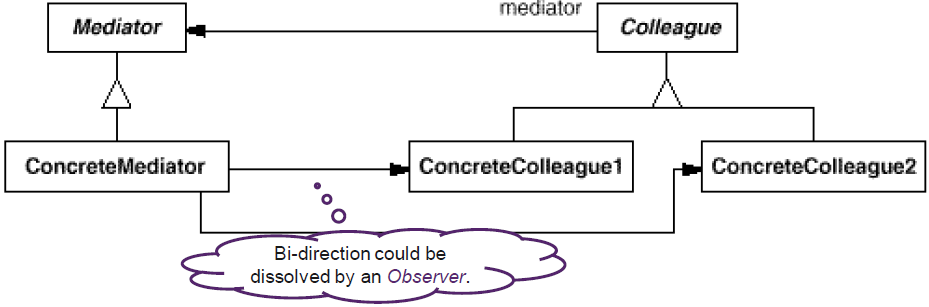
\includegraphics[width=\linewidth]{mediator_static.png}

\textbf{Dynamics}

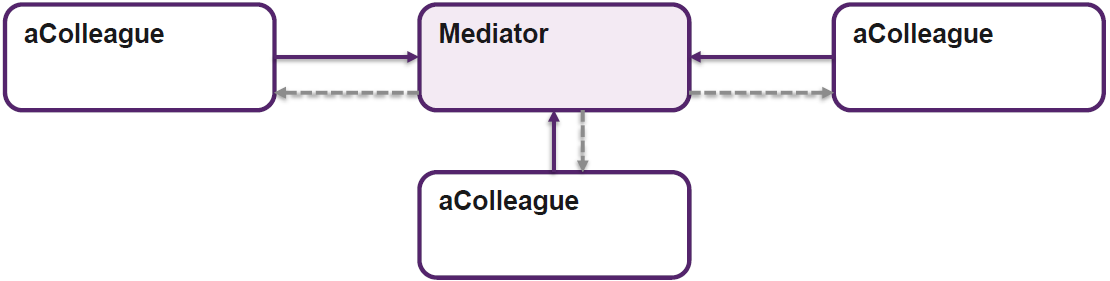
\includegraphics[width=\linewidth]{mediator_dynamic.png}

\subsubsection{Problem}
\begin{itemize}
    \item Objektstrukturen können zu vielen Verbindungen zwischen Objekten führen
    \item Im schlimmsten Fall kennt jedes Objekt jedes andere
\end{itemize}

\subsubsection{Intent}

Wie kann eine starke Kopplung zwischen mehreren Objekten vermieden und die Kommunikation vereinfacht werden?

\subsubsection{Solution}

Reduziert chaotische Abhängigkeiten zwischen Objekten. Das Pattern verhindert direkte Kommunikation zwischen den Objekten und zwingt diese mit dem Madiator-Objekt zusammenzuarbeiten.

\textbf{Participants}

\textcolor{blue}{Mediator} kapselt die Interaktion einer Gruppe von Objekten

\textcolor{blue}{Colleagues} Verweis auf Mediator; dies fördert loose coupling

\subsubsection{Consequences}

\textbf{Benefits}

\begin{itemize}
    \item \textcolor{blue}{Single Responsibility Principle}. Kommunikation zwischen verschiedenen Komponenten kann zu einem Ort extrahiert werden. Macht es einfacher diese zu unterhalten
    \item \textcolor{blue}{Open / Closed Principle} Es können neue Mediators hinzugefügt werden, ohne die Komponenten zu ändern
    \item zentralisiert die Steuerung der Kommunikation zwischen Objekten
    \item Reduziert die Kopplung zwischen den Komponenten (Colleagues)
    \item Individuelle Komponenten (Colleagues) können einfacher wiederverwendet werden
\end{itemize}
\vspace{10pt}
\textbf{Liabilities}

\begin{itemize}
    \item erhöht die Komplexität
    \item Single point of failure
    \item Mediator kann zu einer God-Klasse werden (schwer wartbarer Monolith)
\end{itemize}

\subsubsection{Implementation}
\begin{itemize}
    \item Mediator as an Observer
    \item Colleagues act as Subject
\end{itemize}
\vspace{10pt}
\textbf{Known Uses}
\begin{itemize}
    \item Message Bus Systems
    \item Redux Dispatcher
\end{itemize}

\subsection{Memento (Behavioral)}

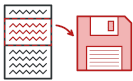
\includegraphics[width=0.2\linewidth]{memento-icon.png}

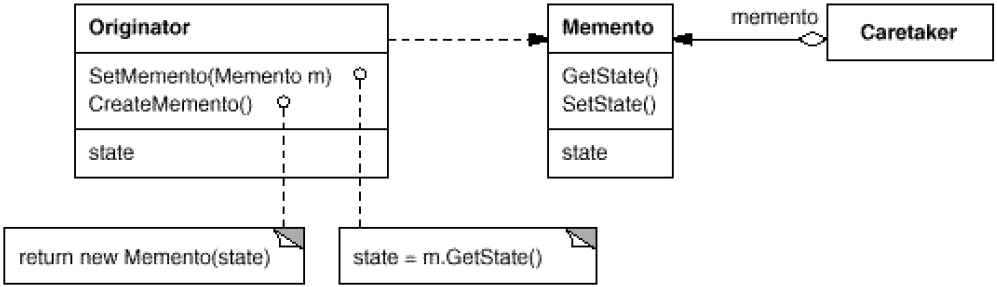
\includegraphics[width=\linewidth]{memento.png} \\

\columnbreak
\textbf{Dynamics}

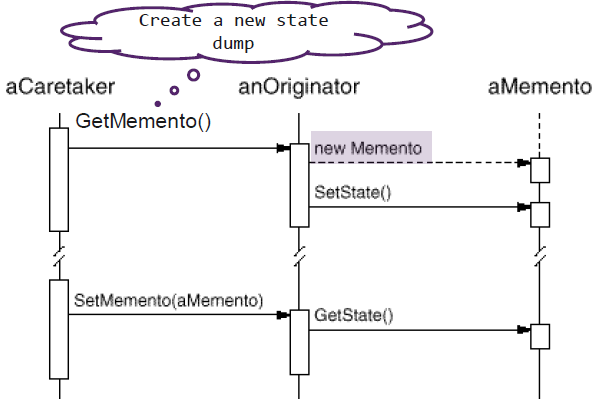
\includegraphics[width=0.7\linewidth]{memento_dynamic.png}

\subsubsection{Problem}
\begin{itemize}
    \item Manchmal ist es notwendig, den internen Zustand eines Objekts aufzuzeichnen
    \item Objekte kapseln normalerweise ihren Zustand und machen ihn unzugänglich.
\end{itemize}

\subsubsection{Intent}

Wie kann der Zustand eines Objekts externalisiert werden, ohne seine Kapselung zu verletzen?

\subsubsection{Solution}

Erlaubt das Speichern und Wiederherstellen von vorherigen Zuständen eines Objekts, ohne die Implementierungs Details zu enthüllen \\

\textbf{Participants}

\textcolor{blue}{Memento} Speichert einige/alle internen Zustände des Originator. Erlaubt nur dem Originator den Zugriff auf seine internen Informationen

\textcolor{blue}{Originator} Kann Memento-Objekte erstellen, um seinen internen Zustand an strategischen Punkten zu speichern und kann seinen eigenen Zustand so wiederherstellen, wie es das Memento-Objekt vorgibt

\textcolor{blue}{Caretaker} Speichert die Memento-Objekte und kann den Inhalt nicht untersuchen / bearbeiten

\subsubsection{Implementation}
\begin{itemize}
    \item Originator creates memento and passes over its internal state
    \item Can be combined with Factory Method
    \item Declare Originator as \textit{friend} of Memento, so Originator can read out its properties
\end{itemize}

\subsubsection{Consequences}
\textbf{Benefits}
\begin{itemize}
    \item Snapshots können erstellt und genutzt werden ohne die Kapselung zu verletzen
    \item Originator Code kann vereinfacht werden, indem der Caretaker Rücksicht auf die History des Originator Zustandes nimmt
\end{itemize}
\textbf{Liabilities}
\begin{itemize}
    \item App kann sehr viel RAM brauchen (erstellt jedes Mal eine komplette Kopie)
    \item Caretakers müssen den Life-Cycle des Originator verfolgen, damit überflüssige Mementos
    gelöscht werden können
\end{itemize}

\subsection{Command (Behavioral)}

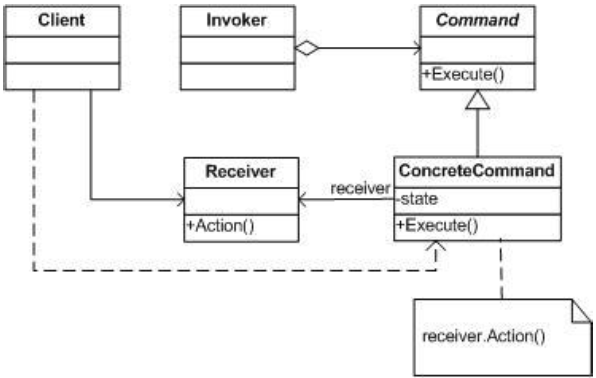
\includegraphics[width=\linewidth]{command.png} \\

\textbf{Dynamics}

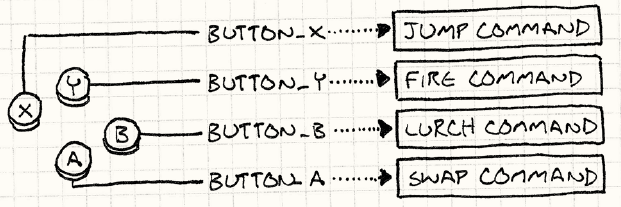
\includegraphics[width=\linewidth]{command_dynamic.png}

\subsubsection{Problem}
\begin{itemize}
    \item Entkoppeln Sie die Entscheidung, was ausgeführt werden soll, von der Entscheidung, wann es ausgeführt werden soll.
    \item Die Ausführung benötigt einen zusätzlichen Parametrisierungskontext
\end{itemize}

\subsubsection{Intent}
Wie können Befehle gekapselt werden, so dass sie parametrisiert, geplant (scheduled), protokolliert (logged) und/oder rückgängig (undo) gemacht werden können?

\subsubsection{Solution}
Wandelt einen Request in ein stand-alone Objekt um, welches alle Informationen zum Request enthaltet. Dies erlaubt, das Requests als Methoden-Argumente verwendet werden, die Request verzögert werden, in einer Warteschlange stehen und erlaubt undoable Operationen.

\subsubsection{Consequences}
\textbf{Benefits}
\begin{itemize}
    \item \textcolor{blue}{Single Responsibility Principle} Klassen die Operationen aufrufen können von den Klassen, die Operationen ausführen, entkoppelt werden
    \item \textcolor{blue}{Open / Closed Principle} Neu Commandos können hinzugefügt werden ohne existierenden Client Code zu zerstören
    \item Undo / Redo kann implementiert werden
    \item Das Ausführen von Operationen kann aufgeschoben werden
    \item Ein Set von einfachen Commands kann zu einem komplexen zusammengestellt werden
\end{itemize}
\vspace{10pt}
\textbf{Liabilities}
\begin{itemize}
    \item Der Code kann komplizierter werden, weil ein neues Layer zwischen Sender und Empfänger
    hinzugefügt wird
\end{itemize}

\subsection{Command Processor (Behavioral)}

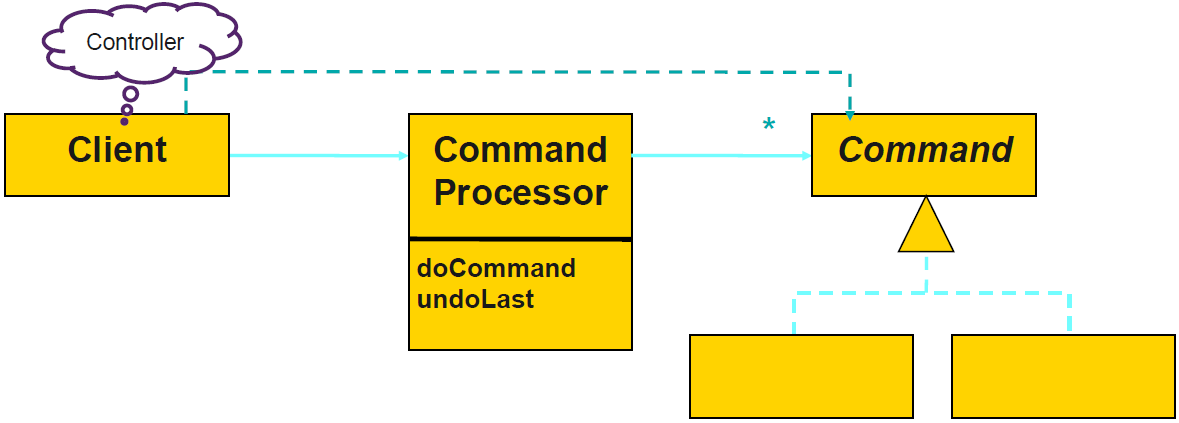
\includegraphics[width=0.8\linewidth]{command_processor.png} \\

\textbf{Dynamics}

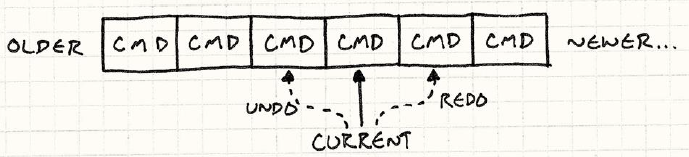
\includegraphics[width=\linewidth]{command_processor_dynamic.png}

\subsubsection{Problem}
\begin{itemize}
    \item Gängige UI-Anwendungen unterstützen \textcolor{blue}{Do} und mehrere \textcolor{blue}{Undo}-Schritte
    \item Schritte vorwärts und rückwärts sind in einer History zugänglich
\end{itemize}

\subsubsection{Intent}
Wie können wir Befehlsobjekte verwalten, so dass die Ausführung von der Anfrage getrennt ist und die Ausführung später rückgängig (undo) gemacht werden kann?

\subsubsection{Solution}
Separiere den Request für einen Service von dessen Ausführung. Command Processor Komponente verwaltet Requests als separate Objekte, plant zeitlich dessen Ausführung und bietet zusätzliche Services, wie das Speichern von Request-Objekten für späters \textcolor{blue}{undo} \\

\textbf{Participants}

\textcolor{blue}{Command Processor} Ein separates Processor object kann die Verantwortung für mehrere Command objects übernehmen

\textcolor{blue}{Command} Eine einheitliche Schnittstelle zur Ausführung von Funktionen

\textcolor{blue}{Controller} Übersetzt Anfragen in Befehle und übermittelt Befehle an den Befehlsprozessor.

\subsubsection{Implementation}
\begin{itemize}
    \item Command Processor contains a \textit{Stack} which holds the command history
    \item Controller creates the Commands and passes them over to Command Processor
    \item Creation of Commands may be delegated to a \textcolor{blue}{Simple Factory}
\end{itemize}

\subsubsection{Consequences}
\textbf{Benefits}
\begin{itemize}
    \item \textcolor{blue}{Flexibility} Command Processor und Controller werden unabhängig von Commands implementiert
    \item Central Command Processor erlaubt zusätzlich Services die der Command-Ausführung zugehören
    \item \textcolor{blue}{Verbessert die Testbarkeit} Command Processor kan verwendet werden, um Regression Tests
    durchzuführen
\end{itemize}
\vspace{10pt}
\textbf{Liabilities}
\begin{itemize}
    \item Effizienz-Verlust wegen zusätzlichen Umwegen
\end{itemize}


\subsection{Visitor (Behavioral)}

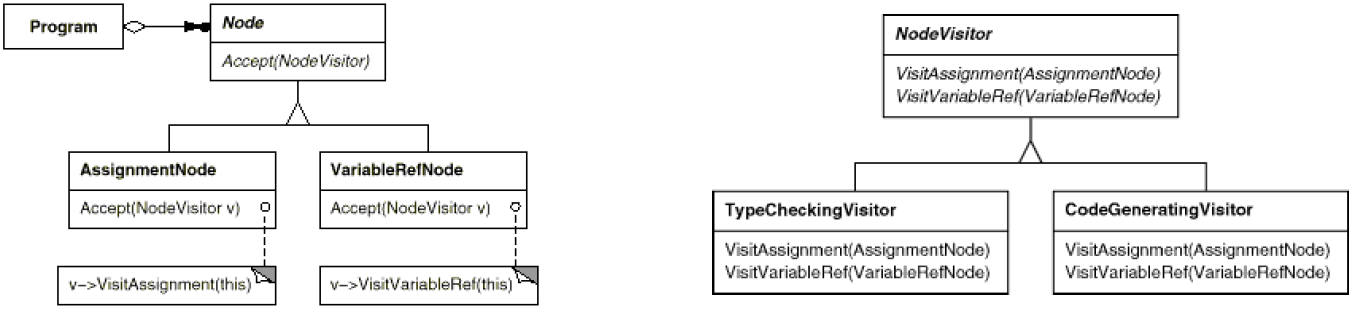
\includegraphics[width=\linewidth]{visitor.png}

\subsubsection{Problem}
\begin{itemize}
    \item Operationen auf bestimmten Klassen müssen geändert/hinzugefügt werden, ohne dass diese Klassen geändert werden müssen
    \item Verschiedene Algorithmen sind für die Verarbeitung eines Objektbaums erforderlich
\end{itemize}

\subsubsection{Intent}
Wie kann das Verhalten einzelner Elemente einer Datenstruktur geändert/ersetzt werden, ohne die Elemente zu ändern?

\subsubsection{Solution}
Represent an operation to be performed on the elements of an object structure. Visitor lets you define a new operation without changing the classes of the elements on which it operates.

\subsubsection{Implementation}
\begin{itemize}
    \item 2 Class Hierarchies (Elements / Visitors)
    \item Visitors iterate though object hierarchy
    \item Solves Double-Dispatch problem of single dispatched programming languages
\end{itemize}
\vspace{10pt}
\textbf{Patterns that combine naturally with Visitor}
\begin{itemize}
    \item Composite
    \item Interpreter
    \item Chain of Responsibility
\end{itemize}

\subsubsection{Consequences}
\textbf{Benefits}
\begin{itemize}
    \item \textcolor{blue}{Open / Closed Principle} Neues Verhalten das auf Objekten unterschiedlicher Klassen ausgeführt werden kann, ohne die Klassen zu ändern
    \item \textcolor{blue}{Single Responsibility Principle} Mehrere Version desselben Verhalten können in die selbe Klasse verschoben werden
    \item Es können komplexe Datenstrukturen traversiert werden
\end{itemize}
\vspace{10pt}
\textbf{Liabilities}
\begin{itemize}
    \item Alle Visitors müssen updatet werden, wenn eine Klasse hinzugefügt oder entfernt wird
    \item Visitors können nicht auf private Felder zugreifen
    \item Visiting Sequence ist innerhalb von Nodes fix definiert
    \item Visitor zerlegt die Logik
\end{itemize}
